\chapter{PyBEL: a computational framework for Biological Expression Language}
\label{ch:pybel}

\section*{Preface}

While \ac{BEL} had been previously demonstrated to support the combination of data and knowledge in analyses~\cite{Martin2012,Laifenfeld2012,Catlett2013,Martin2014,Vasilyev2014,Laifenfeld2014}, its surrounding computational ecosystem was incredibly limited.
The previously existing software provided by Selventa, the original developer of BEL, was aging and not amenable to extension or interactive computational investigation that is becoming mainstream with the advent of the Jupyter Notebook~\cite{Kluyver2016}.
In order to leverage the unique ability of \ac{BEL} to integrate multi-scale and multi-modal knowledge to support downstream simulation, target prioritization, mechanism of action deconvolution, and other methods, it was necessary to build a new ecosystem that is presented in the following paper.

\vspace*{\fill}

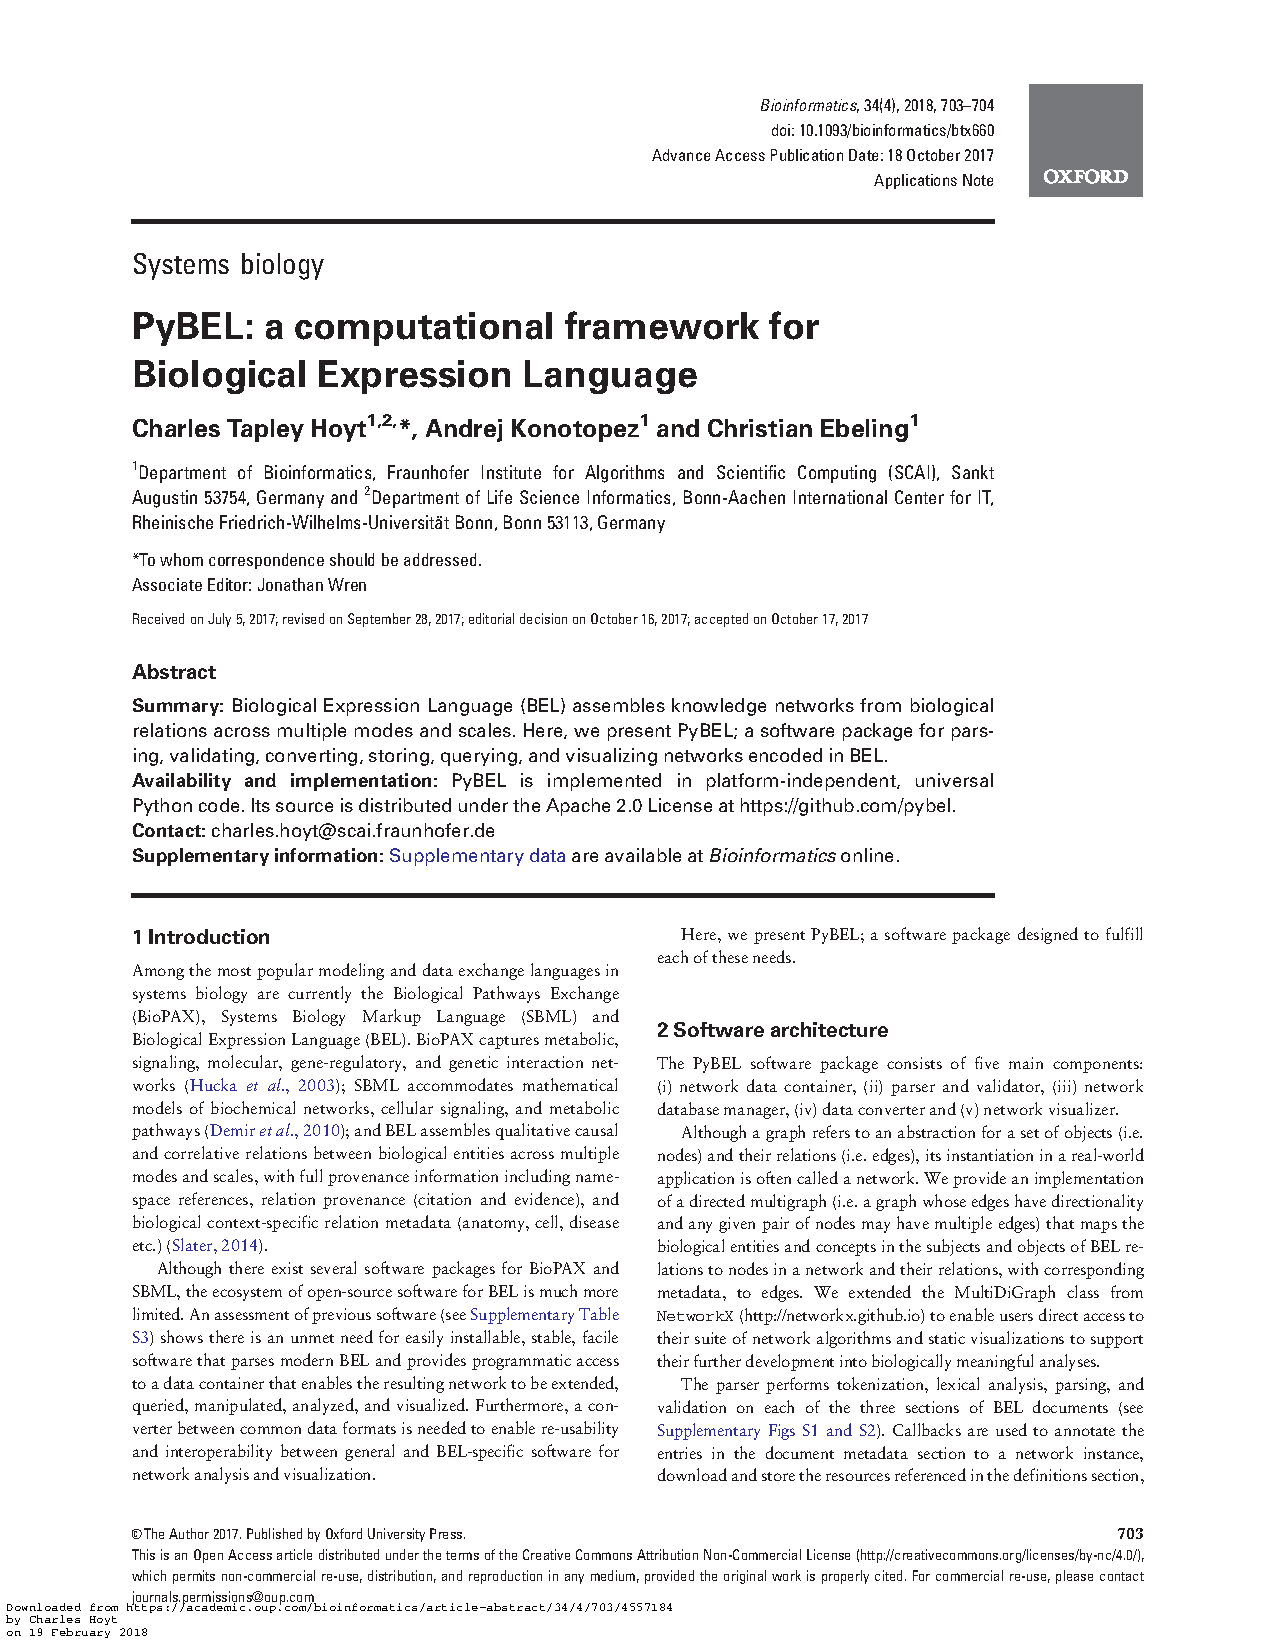
\includepdf[pages={-}]{articles/pybel.pdf}

\section*{Postface}

In order to make the PyBEL ecosystem sustainable, it was made open source, easily installable, integrated with existing systems in systems and networks biology, tested, and well-documented.
It was then demonstrated the ease with which \ac{BEL} could be used in the Python environment as well as presented a implementation of a variant of the heat diffusion algorithm described by~\cite{Leiserson2015}.

While PyBEL contained several imports and exports for other software used by systems and network biologists, it still lacked an accessible interface for biologists.
It was also alluded that knowledge from structured sources could be integrated, especially from other standards like \ac{BioPAX} and \ac{SBML}.
Each of these are addressed in Chapters~\ref{ch:belcommons}, ~\ref{ch:recuration}, and ~\ref{ch:bio2bel}.
